\documentclass{article}

\usepackage[T1]{fontenc}
\usepackage[polish]{babel}
\usepackage[utf8]{inputenc}
\usepackage{amsmath}
\usepackage{hyperref}
\usepackage{tablefootnote}
\usepackage{graphicx}
\graphicspath{ {./media/} }
\begin{document}

\section{Cel ćwiczenia}
Celem ćwiczenia było wyznaczenie współczynnika sprężystości sprężyn przy użyciu metody statycznej i dynamicznej.  Ćwiczenie obejmowało również wyznaczenie współczynnika sprężystości dla układu sprężyn połączonych równolegle i szeregowo. Podczas opracowania przyjęliśmy $\Delta x = 2$ mm chcąc uwzględnić podziałkę linijki oraz drobną oscylację ciężarka, a także $\Delta m = 0$, 
ponieważ odczytywaliśmy masę z oznaczeń na ciężarkach oraz $\Delta t = 0,5 $ s.

\section{Metoda statyczna}
\subsection{pomierzone dane}
\begin{center}
\begin{tabular}{ c | c | c | c}
l.p. & m [g] & $x_1$ [cm] & $x_2$ [cm]\\
\hline
 1    & 50 & 3,7 & 5.1\\ 
 2    & 100 & 6,7 & 10,3\\ 
 3  & 150 & 10,3 & 15,5\\ 
 4  & 200 & 13, 9 & 20,6\\
 5   & 250 & 17,0 &25,8\\
 6  & 300 & 20,6 & 31,0\\
 7  & 350 & 24,7 & 36,1\\
 8  & 400 & 27,7 & 41,3\\
 9  & 450 & 31,3 & 46,4

\end{tabular}
\end{center}
$m$ - masa zawieszona na sprężynie \\
$x_i$ - zmiana wychylenia i-tej sprężyny od wychylenia początkowego po zawieszeniu ciężarków o określonej masie

\subsection{wykres $x_1(m)$}
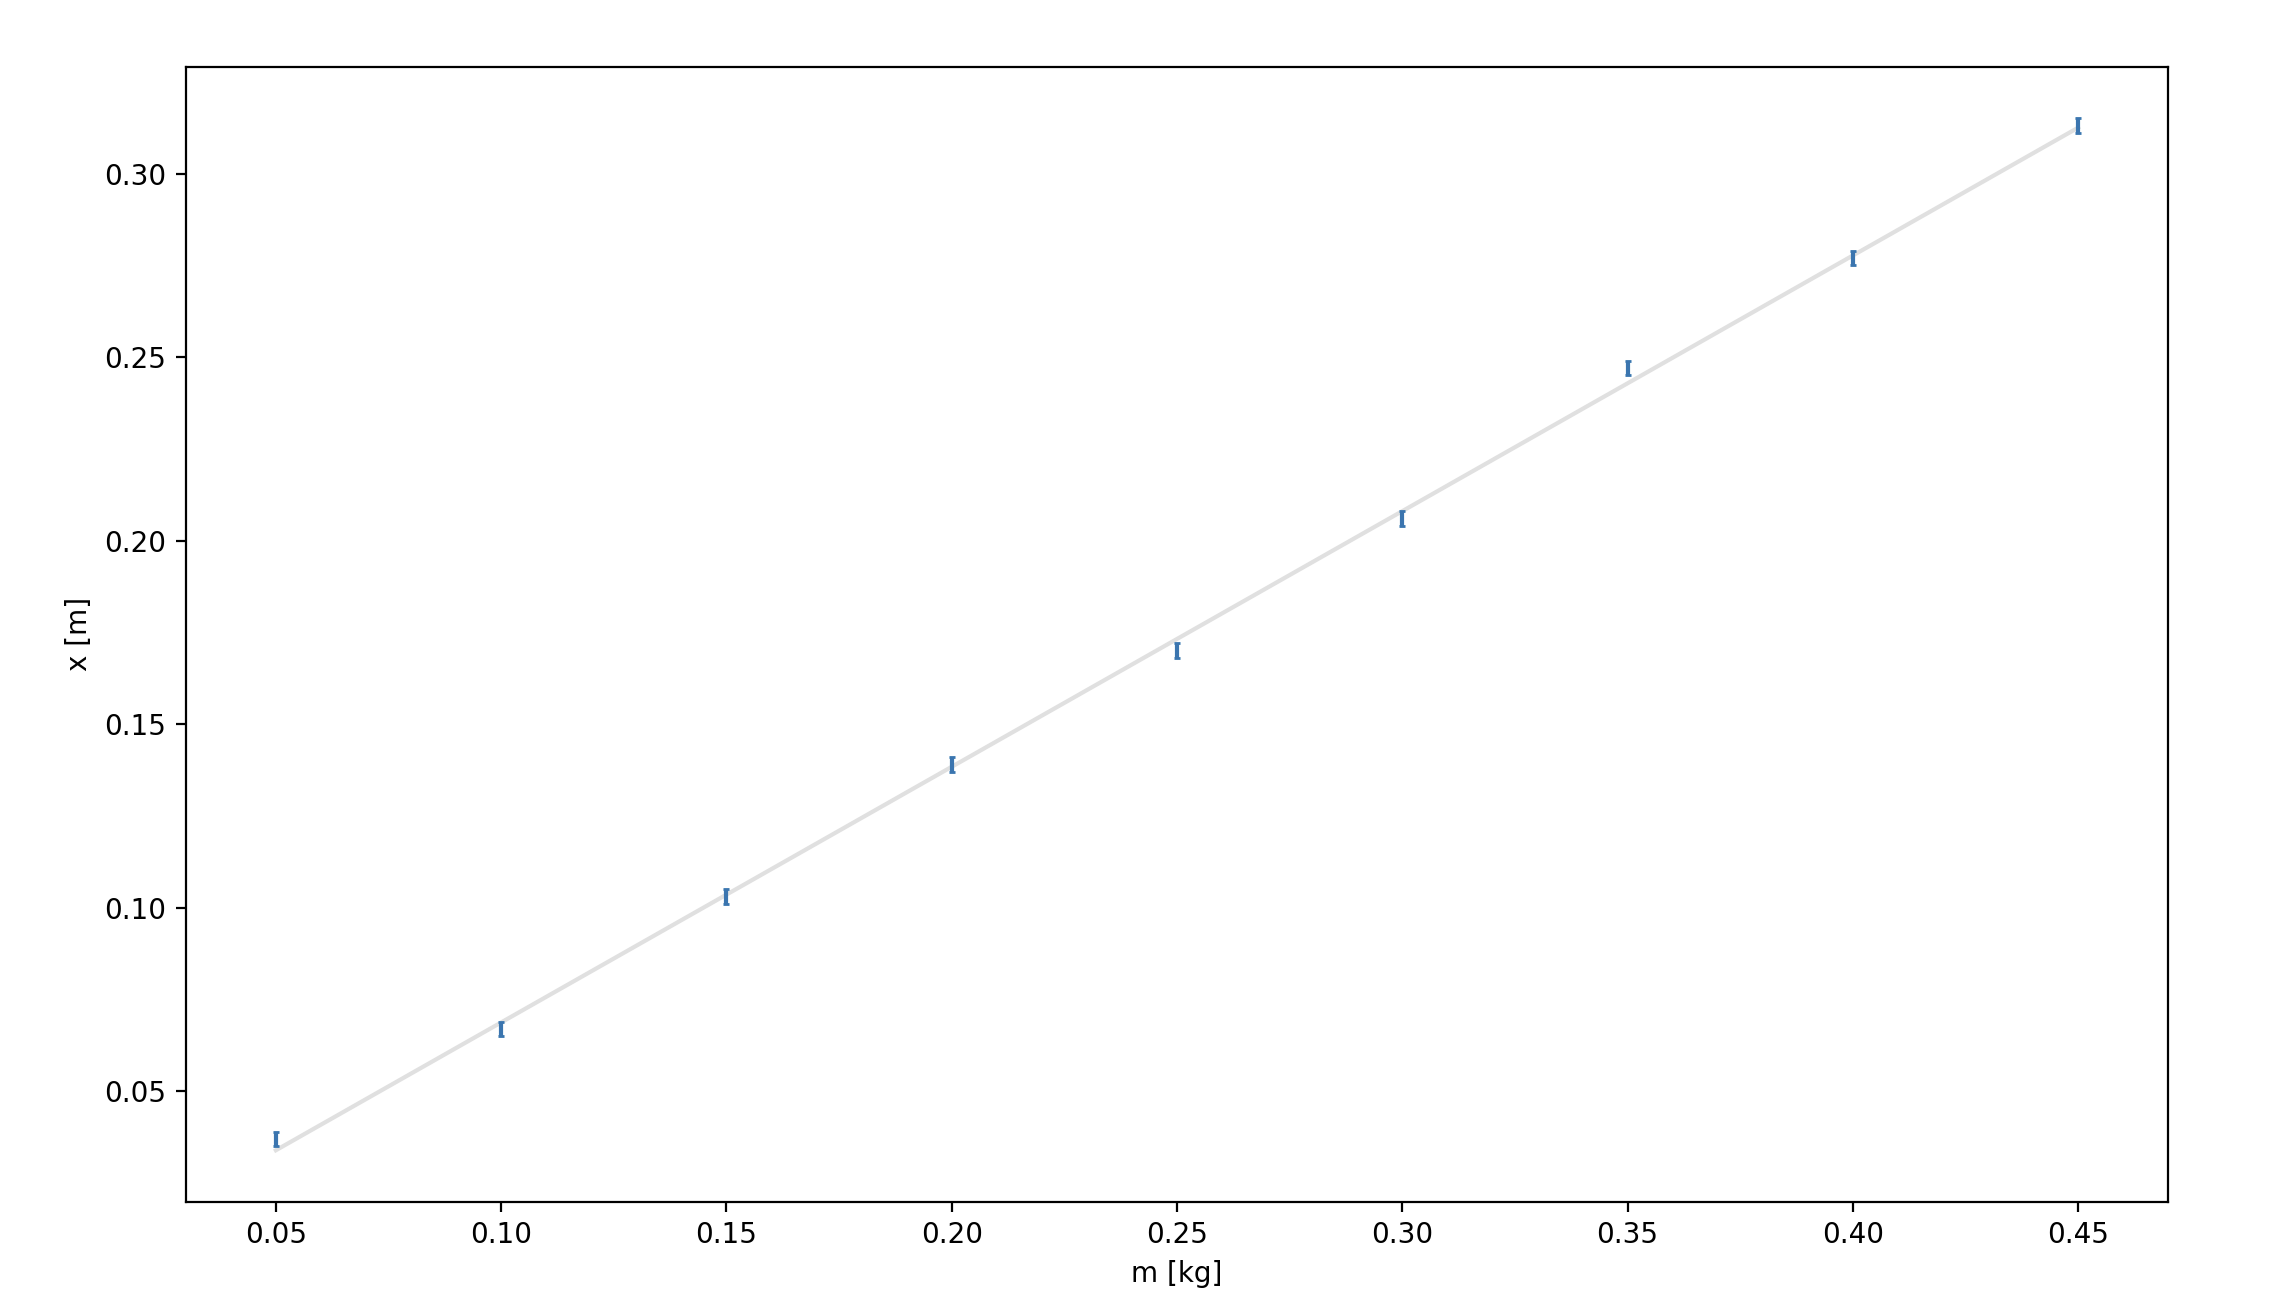
\includegraphics[width=15cm]{m7_1}\\
 $a = 0.69$  - wartość współczynnika kierunkowego prostej otrzymanej metodą regresji liniowej
\subsection{wykres $x_2(m)$}
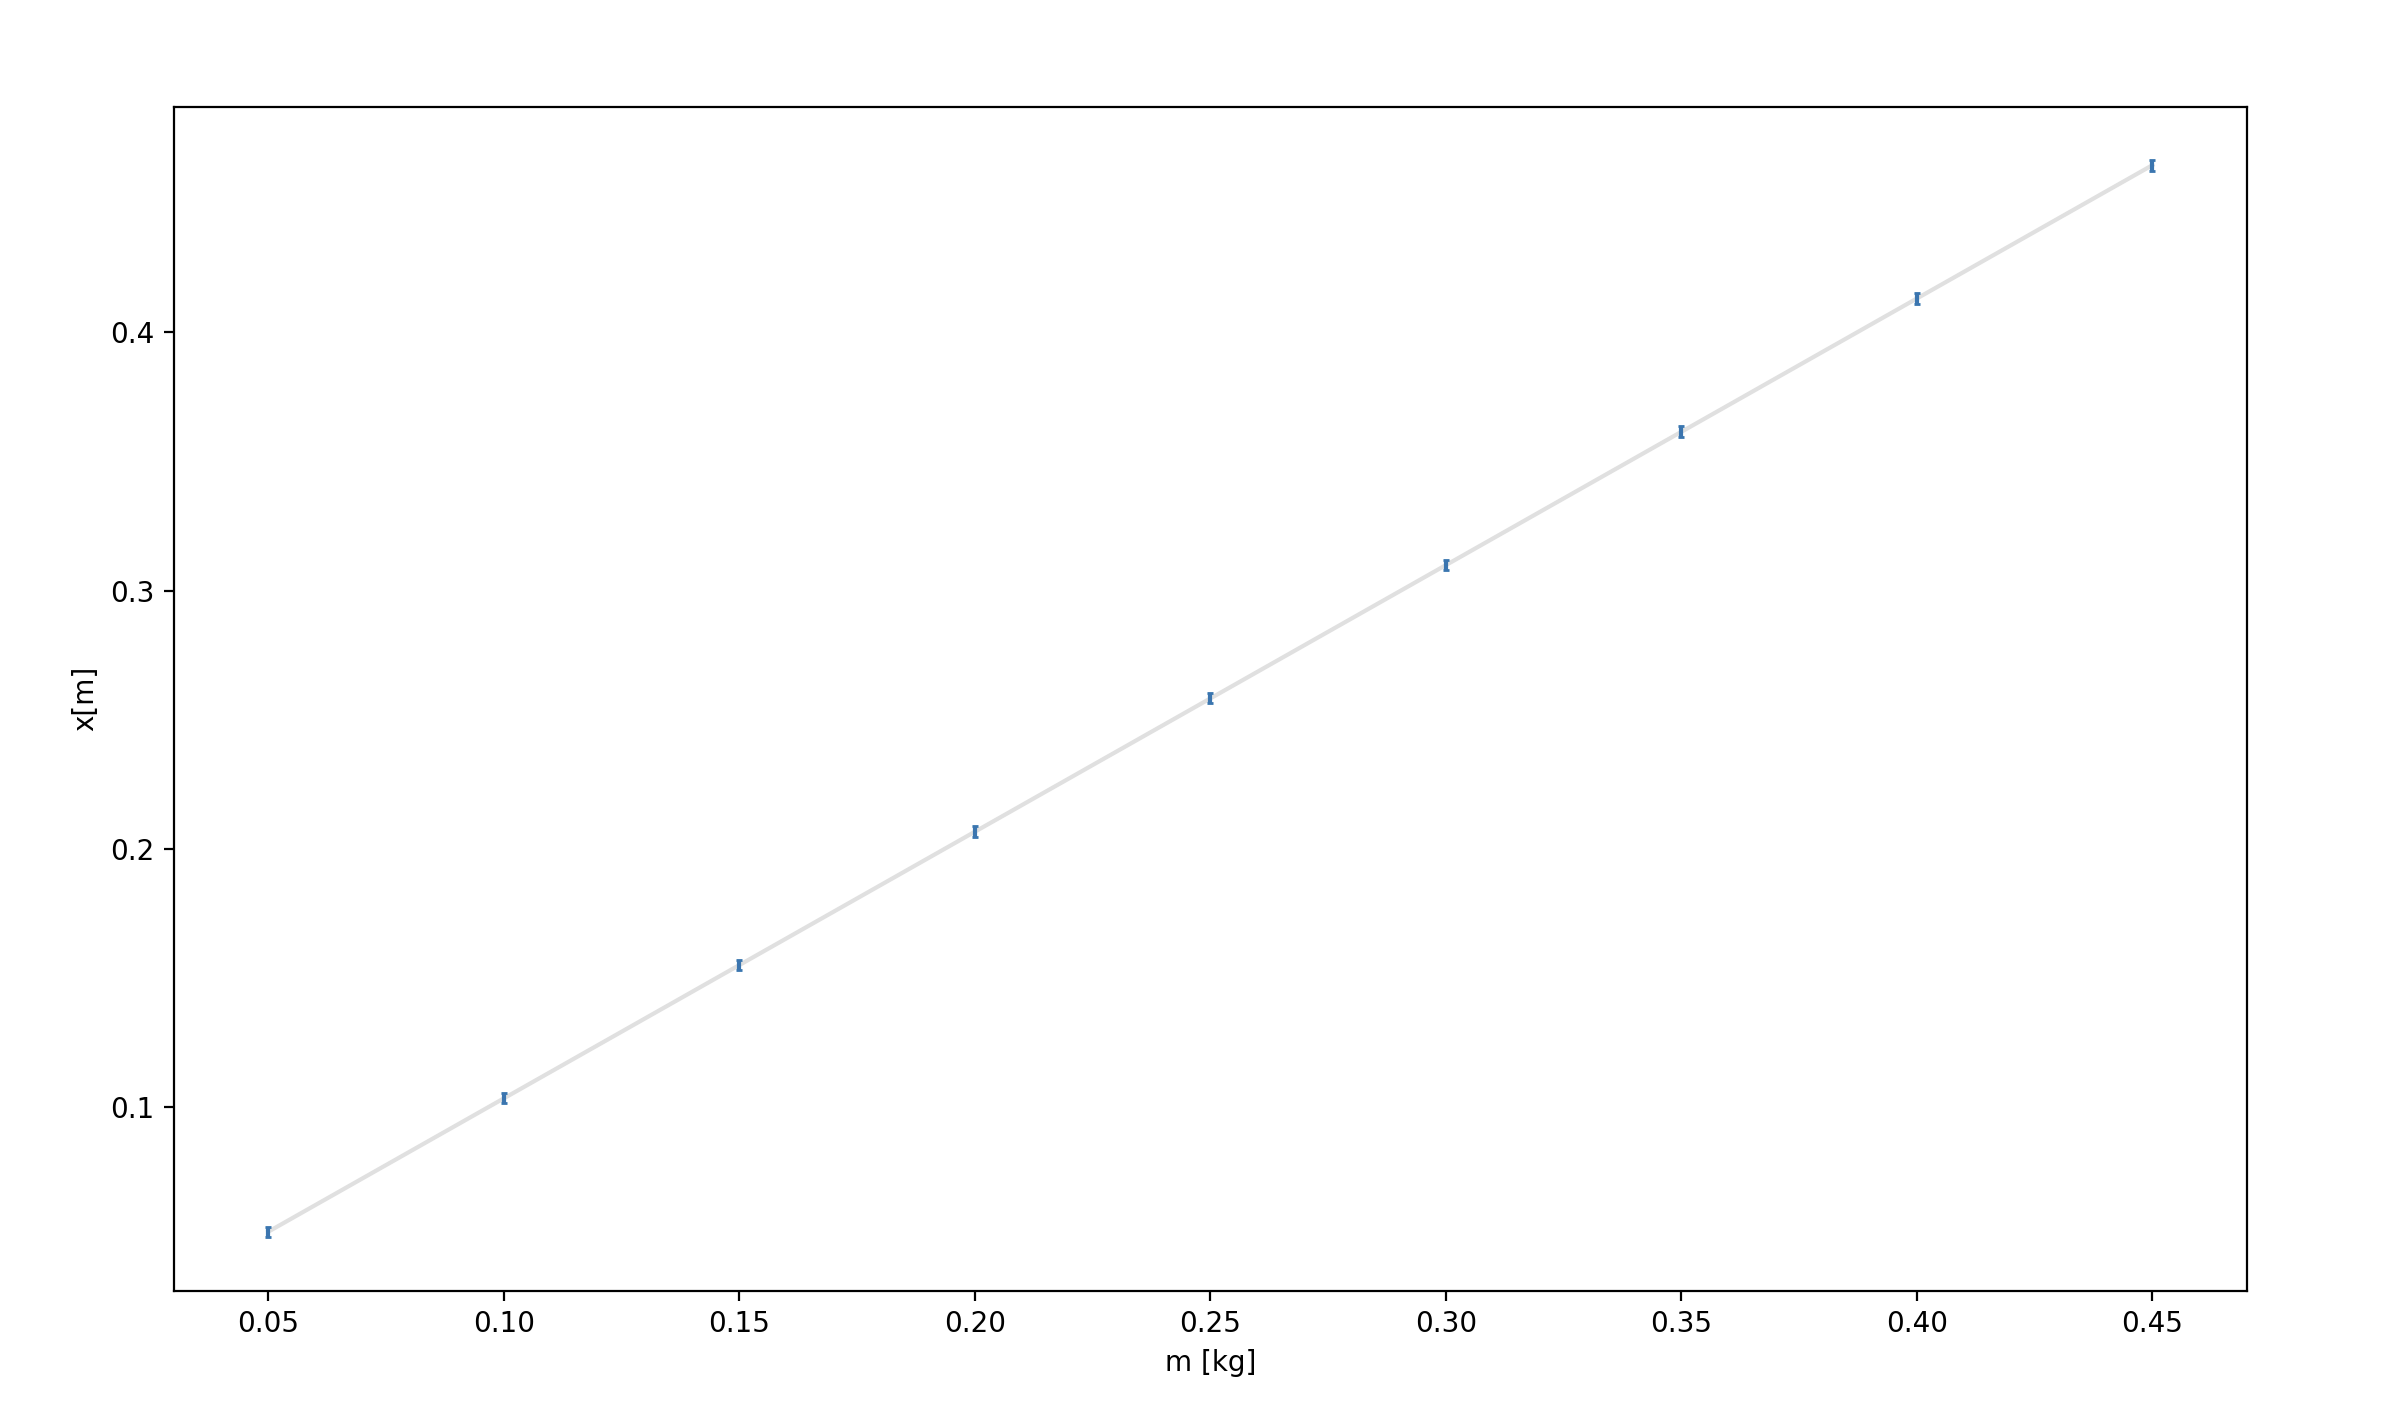
\includegraphics[width=15cm]{m7_1_2}
$a = 1.03$ - wartość współczynnika kierunkowego prostej otrzymanej metodą regresji liniowej
\subsection{obliczenie stałej sprężystości}
korzystamy ze wzoru\footnote{\url{https://pg.edu.pl/files/ftims/2021-03/Cwicz63_02.pdf} (63.15)}
\begin{gather*}
	k = \frac{g}{a}
\end{gather*} 
gdzie $g = 9,815  \frac{N}{kg}$ - przyspieszenie grawitacyjne ziemi\\
zatem $k_1=14,1 \frac{N}{m}$, $k_2 = 9,5 \frac{N}{m}$

\subsection{rachunek niepewności}

Do wyliczenia niepewności k korzystamy ze wzorów \footnote{\url{https://ftims.pg.edu.pl/documents/10673/20436990/wstep.pdf} (42)} \footnote{\url{https://pg.edu.pl/files/ftims/2021-03/Cwicz63_02.pdf} (63.16)}
\begin{gather*}
S_a = \sqrt{\frac{n}{n-2} * \frac{\Sigma y_i^2 - a\Sigma x_iy_i}{n\Sigma x_i^2}} \\
S_k = \frac{gS_a}{a^2}
\end{gather*}
otrzymujemy $S_{k1} = 0,33$ [N/m],  $S_{k2} = 0,10$ [N/m]

\section{Metoda dynamiczna}
\subsection{pomierzone dane}
\begin{center}
\begin{tabular}{ c | c | c| c |c|c}
l.p.  & m [g] & $t_1$ [s]  & $T_1^2$ [$s^2$] & $t_2$ [s] & $T_2^2$ [$s^2$]\\
\hline
 1   & 50 & 8,07 & 0,16 & 9,51 & 0,23\\ 
 2   & 100 & 10,64 & 0,28 & 12,12 & 0,38\\ 
 3   & 150 & 12,55 & 0,39 & 16,03 & 0,64\\ 
 4  & 200 & 15,19 &0,58& 18,55 & 0,86\\
 5  & 250 & 16,66 & 0,69 & 20, 11 & 1,01\\
 6  & 300 & 17,94 & 0,80 & 22, 87 & 1,31\\
 7  & 350 & 19,85 & 0,99 & 24, 14 & 1,46\\
 8  & 400 & 21,41 & 1,15& 25,23 & 1,59\\

\end{tabular}
\end{center}
$m$ - masa zawieszona na sprężynie \\
$t_i$ - pomierzony czas 20 okresów \\
$t_i = 20T_i$

\subsection{wykres $T_1^2(m)$}

\includegraphics[width=15cm]{m7_2}\\

\subsection{wykres $T_2^2(m)$}
\includegraphics[width=15cm]{m7_2_2}

\subsection{obliczenie stałej sprężystości}

korzystamy ze wzoru\footnote{\url{https://pg.edu.pl/files/ftims/2021-03/Cwicz63_02.pdf} (63.17)}
\begin{gather*}
	k = \frac{4\pi^2}{a}
\end{gather*} 
otrzymujemy $k_1=14,14 \frac{N}{m}$, $k_2 = 9,67 \frac{N}{m}$
\subsection{rachunek niepewności}
przyjęliśmy $\Delta t = 0,5s \rightarrow \Delta T = 0,025s$  \\
do wyliczenia niepewności korzystamy ze wzoru \footnote{\url{https://pg.edu.pl/files/ftims/2021-03/Cwicz63_02.pdf} (63.18)}
\begin{gather*}
	S_k = \frac{4\pi^2 S_a}{a^2}
\end{gather*} 
co daje nam $S_{k1} = 0,32$, $S_{k2} = 0,46$

\section{Moduł sztywności}
\subsection{pomierzone dane}
\begin{center}
\begin{tabular}{ c | c  | c}
dana & wartość$_1$\\
\hline
 r & 0,35mm \\
 R & 7,05mm \\ 
 N & 80 zwojów \\ 

\end{tabular}
\end{center}
$r$ - promień drutu sprężyny \\
$R$ - promień sprężyny \\
$N$ - liczba zwojów sprężyny \\
zmierzyliśmy sprężynę 1

\subsection{obliczenie modułu sztywności}
korzystamy ze wzoru\footnote{\url{https://pg.edu.pl/files/ftims/2021-03/Cwicz63_02.pdf} (63.19)}
\begin{gather*}
	G =  \frac{4NR^3k}{r^4}
\end{gather*} 
przyjmując k = $k_{d1}$ - $k_1$ z metody dynamicznej \\
otrzymujemy $G = 105,62 $ GPa \\


\subsection{rachunek niepewności}
do wyliczenia niepewności korzystamy ze wzoru \footnote{\url{https://pg.edu.pl/files/ftims/2021-03/Cwicz63_02.pdf} (63.20)}
\begin{gather*}
	|\Delta G| = G*(|\frac{\Delta N}{N}| + |\frac{3\Delta R}{R}| + |\frac{4\Delta r}{r}| + |\frac{\Delta k}{k}|  )
\end{gather*}
gdzie przyjmujemy $\Delta R = \Delta r = 0.05mm$, $\Delta N = 5$, $\Delta k = 3 S_k$ \\
$\Delta G$ = 80\\

\section{Układ sprężyn połączony równolegle}
\subsection{pomierzone dane}
\begin{center}
\begin{tabular}{ c | c | c | c | c}
l.p. & $\Delta x$ [cm] & m [g] & t[s] & $T^2$ [$s^2$]\\
\hline
 1 & 2,2   & 50 & 5,18 & 0,07\\
 2 & 4,3   & 100 & 8,95 & 0,20\\ 
 3 & 6,6   & 150 &10,66 & 0,28\\ 
 4 & 8,8  & 200 & 11,65 & 0,34\\
 5 & 10,9 & 250 & 13,14 & 0,43\\
 6 & 12,7 & 300 & 14,49 & 0,53\\
 7 & 14,6 & 350 & 15,56 & 0,61\\
 8 & 17,1  & 400 & 16,92 & 0,67\\
 9 & 19,2 & 450 & 17,39 & 0,76

\end{tabular}
\end{center}
oznaczenia jak w pozostałych podpunktach

\subsection{wykres i opracowanie $x(m)$}
\includegraphics[width=15cm]{m7_4a}
a = 0,42 zatem k = 23,3, co zgadza się z założeniami teoretycznymi $k\approx k_1 + k_2$ 

\subsection{wykres i opracowanie $T^2(m)$}
\includegraphics[width=15cm]{m7_4b}\\
tym razem $a=1,67$ a zatem $k = 23,75$,  co zgadza się z założeniami teoretycznymi $k\approx k_1 + k_2$ 

\subsection{rachunek niepewności dla metody statycznej}
do wyliczenia niepewności korzystamy z tych samych wzorów co poprzednio i otrzymujemy
$S_k = 1,1$ [N/m]

\subsection{rachunek niepewności dla metody dynamicznej}
do wyliczenia niepewności korzystamy z tych samych wzorów co poprzednio i otrzymujemy
$S_k = 1, 52$ [N/m]

\section{Układ sprężyn połączony szeregowo}
\subsection{pomierzone dane}
\begin{center}
\begin{tabular}{ c | c | c | c | c  }
l.p. & $x$ [cm] & m [g] & t[s]  & $T^2$ [$s^2$]\\
\hline
 1 & 8,8   & 50 & 12,42 & 0,39\\ 
 2 & 18,0   & 100 &17,80 & 0,79\\ 
 3 & 27,1   & 150 & 21,13 & 1,12\\ 
 4 & 35,9  & 200 & 24,49 & 1,50\\
 5 & 44,9 & 250 & 26,1 & 1,70\\


\end{tabular}
\end{center}
oznaczenia jak w pozostałych podpunktach

\subsection{wykres i opracowanie $x(m)$}
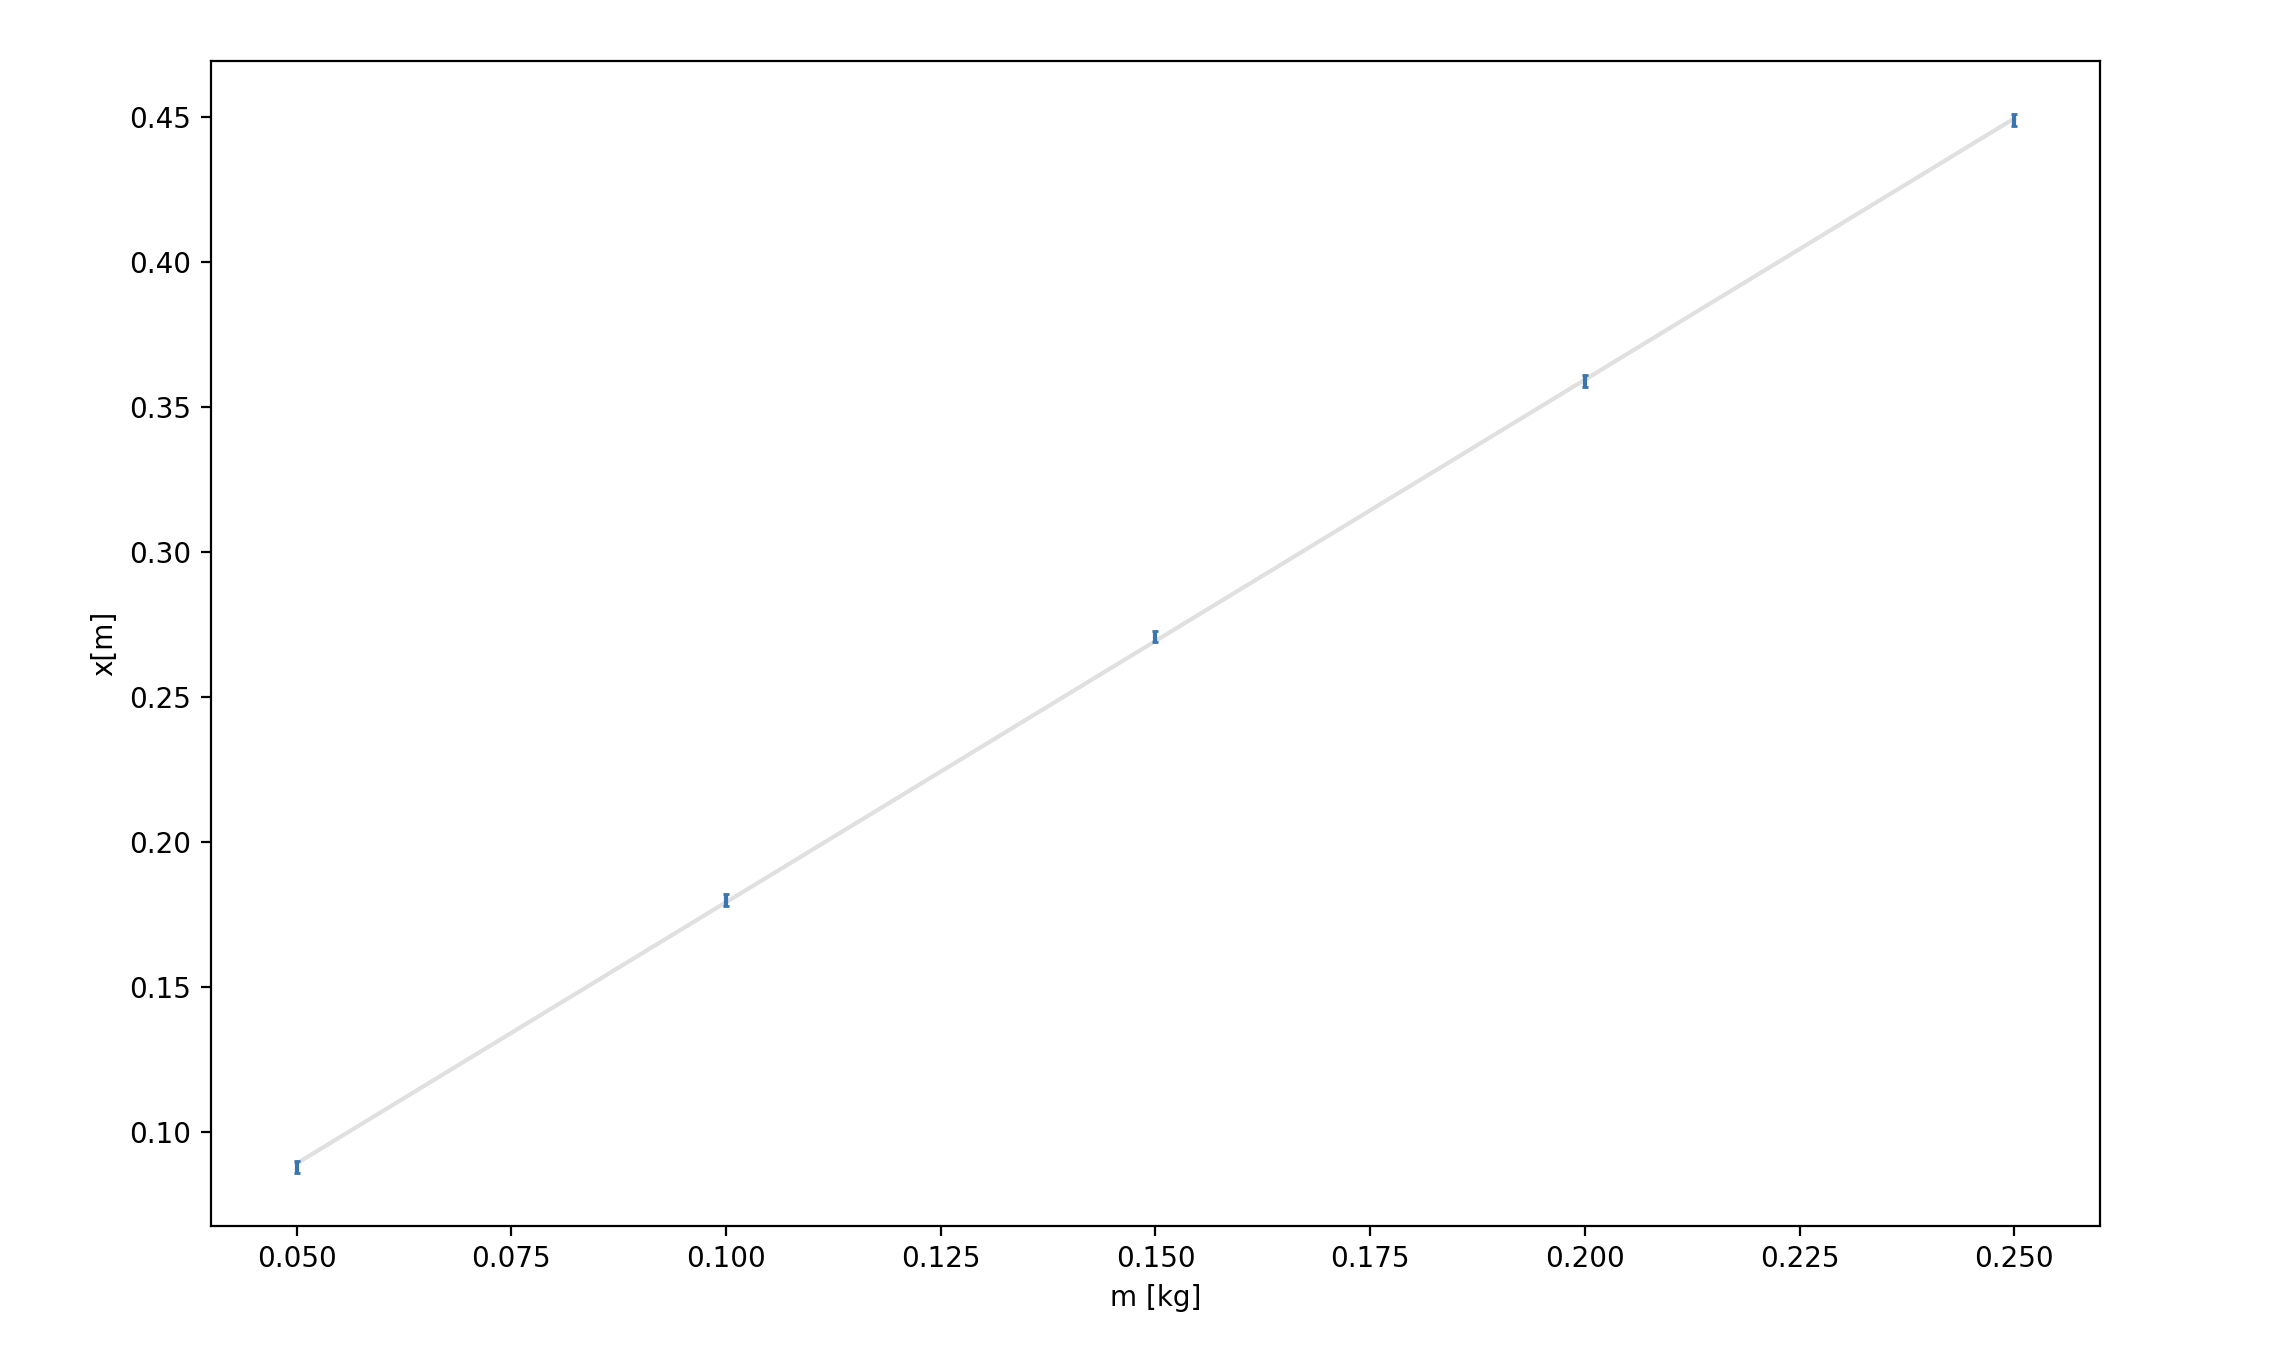
\includegraphics[width=15cm]{m7_5a}
a = 1,80 zatem k = 5,5 co zgadza się z teoretycznymi przewidywaniami, bo $1/k \approx 1/k_1 + 1/k_2$

\subsection{wykres i opracowanie $T^2(m)$}
\includegraphics[width=15cm]{m7_2_2}
a = 6,68 zatem k = 5,90 co zgadza się z teoretycznymi przewidywaniami, bo $1/k \approx 1/k_1 + 1/k_2$

\subsection{rachunek niepewności dla metody statycznej}
do wyliczenia niepewności korzystamy z wyżej wymienionych wzorów i otrzymujemy 
$S_k = 0,2 $[N/m]

\subsection{rachunek niepewności dla metody dynamicznej}
do wyliczenia niepewności korzystamy z tych samych wzorów co poprzednio i otrzymujemy
$S_k = 1, 01$ [N/m]


\section{Wnioski}

\begin{center}
\begin{tabular}{ c | c }
zadanie & współczynnik spreżystości [$\frac{N}{m}$]  \\


\hline
 metoda statyczna  & 14,1 i 9,5\\  
 metoda dynamiczna & 14,14 i 9,67 \\
 układ połączony równolegle& 23,3 i 23,75 \\
 układ połączony szeregowo & 5,5 i 5,90 
\end{tabular}
\end{center}

\begin{center}
	moduł sztywności G = 105,62 GPa
\end{center}

Korzystając z metody statycznej i dynamicznej do wyznaczenia współczynnika sprężystości badanych sprężyn otrzymaliśmy zbliżone do siebie wartości współczynników z obu metod. Z wykresów przedstawiających zależność wychylenia od masy obserwujemy linowy wzrost wychylenia. Co więcej, w przypadku metody dynamicznej tworząc wykres zależności kwadratu okresu drgań od obciążenia również otrzymujemy zależność liniową. W obu przypadkach zaobserwowaliśmy jedynie zakres stosowności prawa Hook`a, nie doprowadzając tym samym sprężyn do zakresu nieliniowych odkształceń nietrwałych i plastycznych. Taką samą sytuację obserwujemy dla układów sprężyn ( szeregowego i równoległego).
W połączeniu szeregowym i równoległym sprężyn uzyskujemy wyniki zbliżone do założeń teoretycznych tych połączeń. Współczynnik sprężystości dla układu szeregowego wzrósł, zaś dla układu równoległego zmalał względem współczynnika pojedynczej  sprężyny.\\ \\
W metodzie statycznej głównym czynnikiem wpływającym na błędy był błąd paralaksy, dokładność linijki oraz minimalne drgania podczas odczytu wartości. W metodzie dynamicznej był to czas reakcji przy pomiarach okresu drgań, a przy obliczaniu modułu sztywności dokładność suwmiarki.\\ \\
Podczas obliczeń przyjęliśmy, że badane sprężyny są nieważkie oraz zaniedbaliśmy opory ruchu.
Wszystkie pomiary zostały wykonane w temperaturze pokojowej.



\end{document}